%---------- Inleiding ---------------------------------------------------------

\section{Introductie}%
\label{sec:introductie}

Op vlak van mobiele app-ontwikkeling is er altijd een tweestrijd tussen het ontwikkelen voor Android en/of iOS. De meeste Android applicaties worden geschreven met een combinatie van Java en Kotlin, terwijl iOS applicaties geschreven zijn in de door Apple ontwikkelde programmeertaal Swift. Het ontwikkelen voor beide platformen op een Native-aanpak voor dezelfde applicatie is echter een kostelijke en tijdrovende onderneming. Het Native programmeren, d.w.z. het ontwikkelen van een applicatie specifiek bedoeld om te draaien op een bepaald platform, zorgt ervoor dat Swift-applicaties niet kunnen draaien op Android-platformen en omgekeerd. Vandaar het kostelijke aspect bij de ontwikkeling voor beide platformen.

Cross-platform ontwikkelen biedt een oplossing voor dit probleem. De applicatie wordt hierbij één keer geschreven en kan vervolgens op verschillende platformen draaien. Dit kan geprogrammeerd worden in talen die op verschillende platformen kunnen draaien, zoals bijvoorbeeld JavaScript en C\verb*|#|. Hierbij is het grote nadeel dat de applicatie niet volledig is geoptimaliseerd voor het platform waarop het uiteindelijk zal draaien. Dit kan zelf leiden tot een tragere en dus slechtere gebruikerservaring.

Deze bachelorproef zal zich focussen op het vergelijken van twee cross-platform frameworks, namelijk React Native en Ionic op het Android-platform. React Native is een framework dat ontwikkeld is door Facebook, en Ionic een framework dat ontwikkeld is door Drifty Co. Bij deze vergelijking zal er specifiek gekeken worden naar de performantie van de applicaties op basis van CPU-verbruik, laadtijden en geheugengebruik. De keuze voor deze specifieke frameworks is gebaseerd op hun populariteit, aangezien deze twee een van de meest gebruikte cross-platform tools zijn. Beiden zijn bovendien open-source en gratis te gebruiken, wat de toegankelijkheid juist vergroot voor software-ontwikkelaars.

Hiervoor zal er een Proof-of-Concept worden uitgevoerd waarbij er een identieke applicatie zal worden ontwikkeld in React Native en Ionic. Deze applicatie zal de vorm nemen van een streaming-applicatie die het mogelijk maakt om video's af te spelen. Bij het ophalen van beeldmateriaal is het van belang dat deze beelden zo vlug mogelijk worden ingeladen en met hoge kwaliteit zonder haperingen worden afgespeeld om de gebruikerservaring zo optimaal mogelijk te maken. Hierbij spelen verschillende factoren zoals de internetverbinding en de processorkracht van grote rol om dit te kunnen verwezenlijken. Deze applicaties zullen vervolgens getest worden op kritieke performantie-aspecten die een rol spelen bij streaming, zoals het CPU-gebruik. De resultaten van deze testen zullen tot slot worden geanalyseerd en vergeleken. Er zullen verschillende versies van deze applicaties worden ontwikkeld, bijvoorbeeld werken met lager beeldkwaliteit of lagere processorkracht. Dit om uitvoerig en diepgaand te testen op aparte aspecten om zo een goed beeld te geven waar de oorzaken van eventuele performantieverschillen liggen. Zo kunnen de voor- en nadelen van beide frameworks worden aangehaald. Om ervoor te zorgen dat dit een zo objectief mogelijk beeld geeft, zullen minder belangrijke aspecten die niet bijdragen tot de kern van het onderzoek worden weggelaten. Denk maar aan de snelheid van de internetverbinding die logischerwijs een grote invloed heeft op de laadtijden van video's, maar niet direct gelinkt is aan de performantie van React Native en Ionic. Dit kan dan bijvoorbeeld opgelost worden door dit lokaal te laten draaien of om een soort constante internetverbinding te simuleren.

Het onderzoek is gericht op ontwikkelaars en kleinere of middelgrote softwarebedrijven die met een beperkt budget hun streaming-applicatie op een zo groot mogelijke markt willen uitbrengen. Het onderzoek zal een antwoord bieden op de vraag welk framework het meest geschikt zal zijn voor de ontwikkeling van een performante streaming-applicatie op Android. Dit zal een meerwaarde bieden voor deze doelgroep, aangezien zij op basis van dit onderzoek een weloverwogen keuze kunnen maken voor het ontwikkelen van hun applicatie.

%---------- Stand van zaken ---------------------------------------------------

\section{State-of-the-art}%
\label{sec:state-of-the-art}

\paragraph{Native vs Cross-Platform}
Allereerst is het belangrijk om het verschil tussen native en cross-platform applicaties te omkaderen. Zoals eerder vermeld, verwijst Native programmeren naar het ontwikkelen van een applicatie bedoeld om te draaien op één gekozen platform zoals Windows of Android. Dit betekent dat de applicatie geschreven is in de programmeertaal die specifiek bedoeld is voor het platform waarop het draait. Denk maar bijvoorbeeld aan Java en Kotlin voor Android. Cross-platform tools daarentegen maken gebruik van onafhankelijke frameworks en talen die op verschillende platformen kunnen draaien (bv JavaScript). Deze worden vervolgens omgezet naar Native code en Native componenten specifiek aan het platform \autocite{Bron2}.

Een voorbeeld van een Cross-Platform applicatie is een Hybride applicatie. Hierbij wordt er gesteund op webtechnologieën zoals HTML, CSS en JavaScript. Deze applicatie draait vervolgens in een native container van het specifieke platform. Dit wil zeggen dat de applicatie in de browser-engine van het desbetreffende platform draait \autocite{Bron6}. Bij Android is dit het WebView component, bij iOS wordt het UIWebView component gebruikt \autocite{Bron4}. Aan de hand van een abstractielaag wordt er volgens \textcite{Bron6} vervolgens toegang verkregen tot de interne mogelijkheden van het apparaat via JavaScript-API's. Deze abstractielaag kan echter wel voor tragere prestaties zorgen, vooral op de CPU, aangezien de applicatie niet volledig ``Native'' is en als gevolg niet volledig geoptimaliseerd is \autocite{Bron1}.

\paragraph{React Native vs Ionic}
Voor dit onderzoek is er specifiek gekozen voor React Native en Ionic. Beide zijn cross-platform frameworks die gebruik maken van JavaScript als basis. \textcite{Bron8} is een open-source Hybrid framework ontwikkeld door Drifty Co en laat toe om te werken met populaire JavaScript frameworks zoals Angular, React en Vue. Het biedt een verscheidenheid aan UI-componenten aan die eruit zien en aanvoelen als Native componenten. Tot slot kan Cordova gebruikt worden om de applicatie te compileren naar een native applicatie voor het desbetreffende platform, zoals Android of iOS \autocite{Bron8}.
React Native is, net zoals Ionic, een open-source framework. Het is ontwikkeld door Facebook en laat toe om te werken met React \autocite{Bron1}. Volgens \textcite{Bron3} en \textcite{Bron2} bleek al snel dat er een paar misconcepties zijn over React Native. Zo wordt het vaak verkeerd beschouwd als een volledig ``Native'' framework. Het is en blijft Hybrid door het gebruik van JavaScript- en JSX (een extensie van JavaScript) componenten. Het ``Native'' aspect in de naam verwijst naar het feit dat het framework gebruik maakt van Native UI-elementen en soms toelaat bepaalde delen van de applicatie in de Native taal te schrijven. Dit zorgt ervoor dat de applicatie sneller kan worden gecompileerd en bijgevolg ook sneller kan draaien. Het is als het ware een brug tussen een Native en Hybrid framework. Vandaar dat dit soms verkeerd wordt gecategoriseerd.

\paragraph{Architectuur van Android}

Verder zal het onderzoek zich ook focussen op de implementatie op het Android-platform. Hierbij is het belangrijk om de architectuur van Android te begrijpen om dit te kunnen linken aan de resultaten die in de Proof-of-Concept zullen worden verkregen. Zo kunnen er logische verklaringen worden gegeven voor eventuele performantieverschillen tussen beide frameworks.

Het Android platform is een mobiele architectuur ontwikkeld door Google. Deze wordt opgedeeld in de volgende lagen:

\begin{figure}
  \centering
  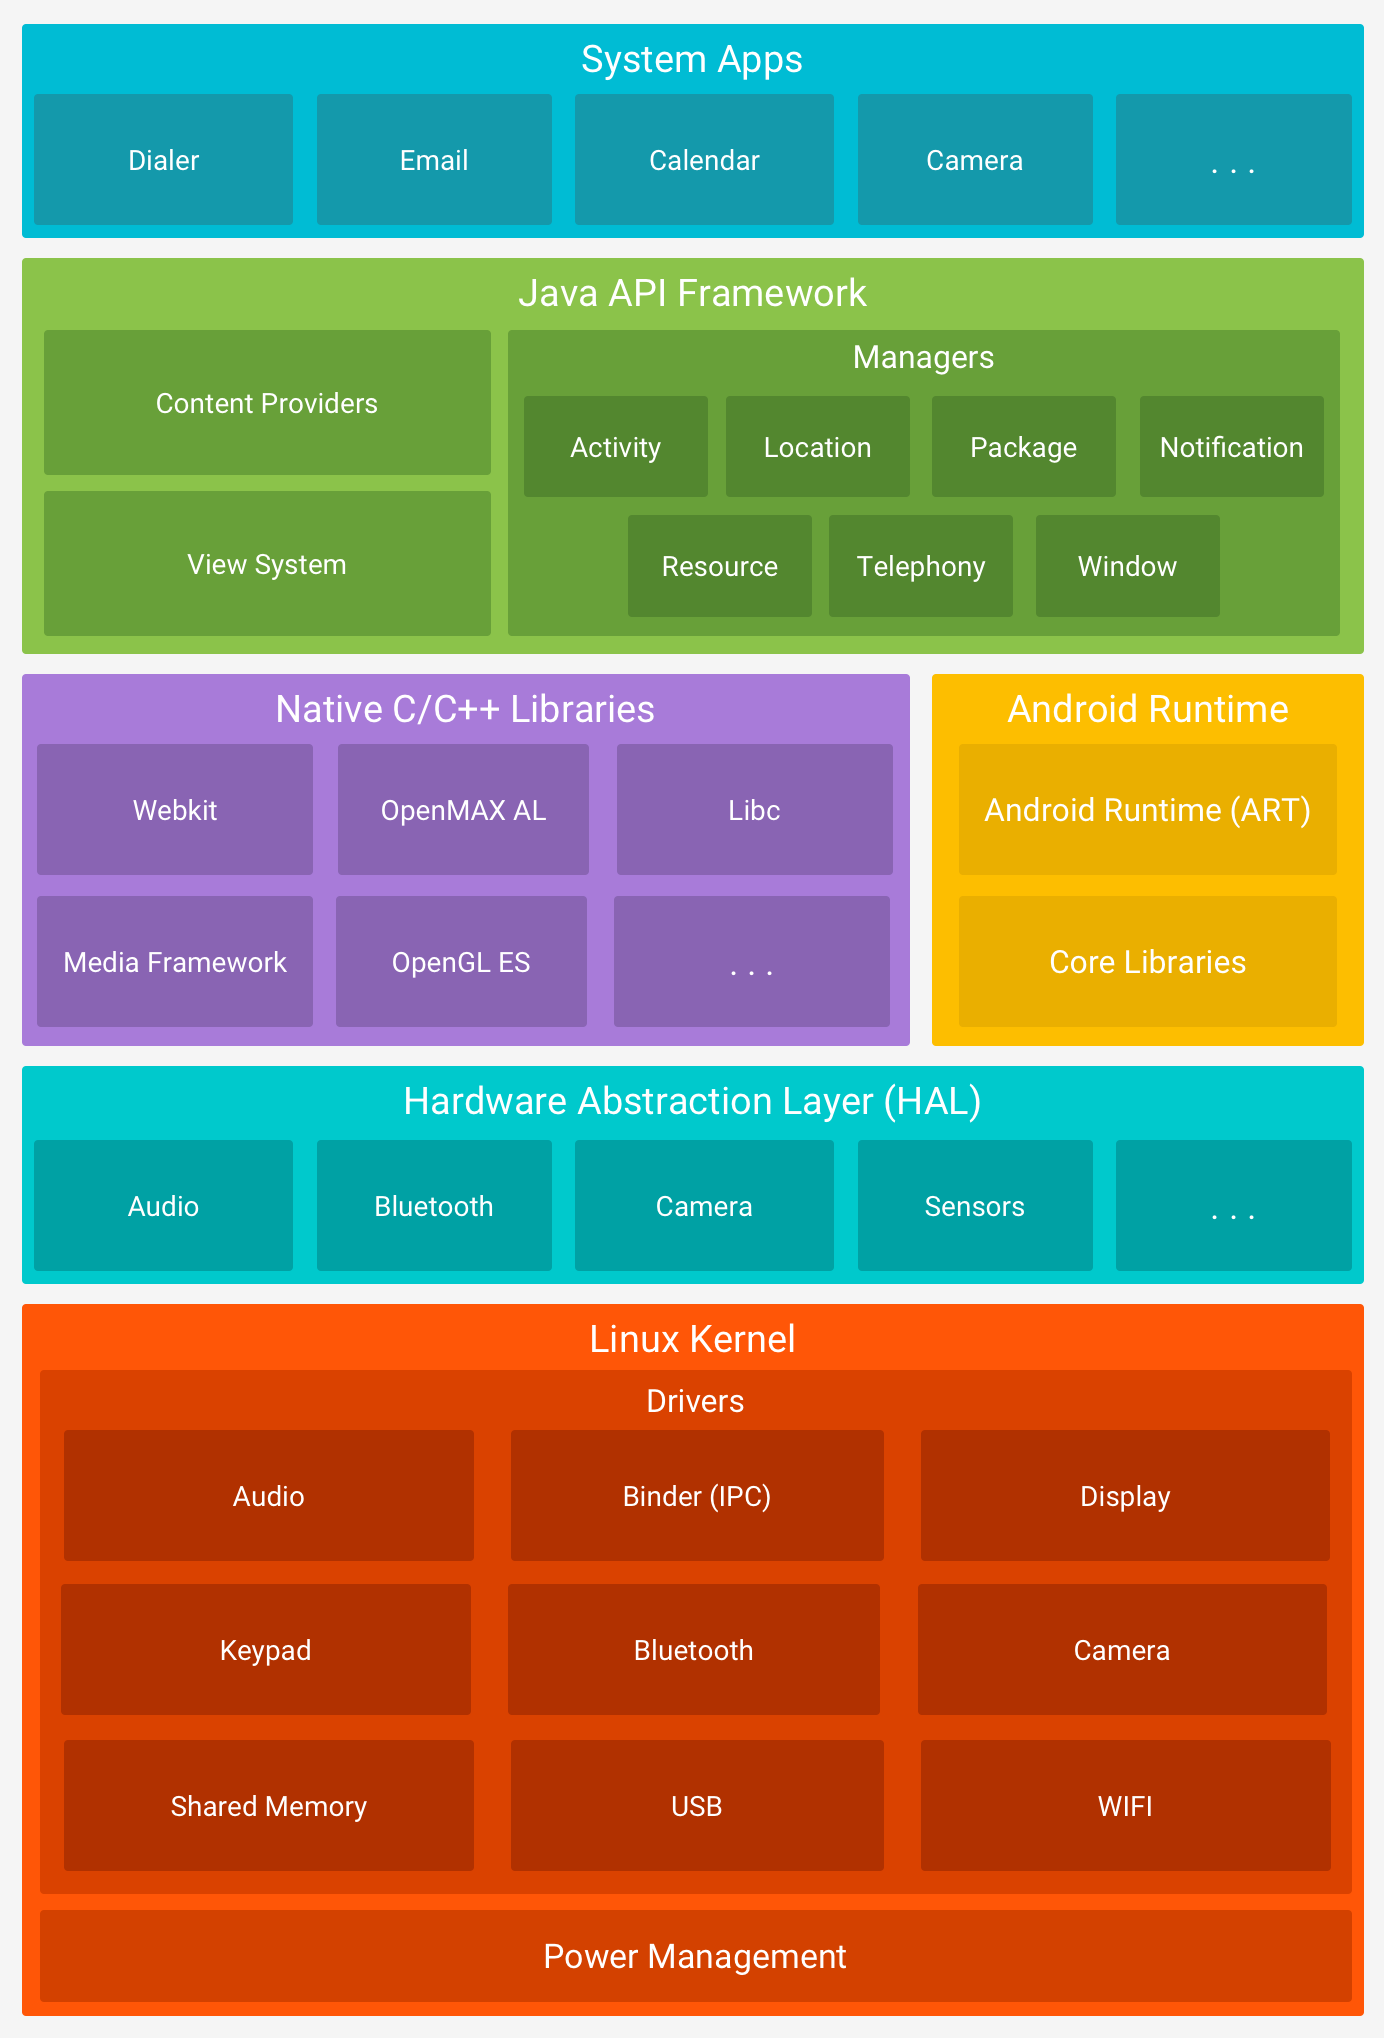
\includegraphics[width=0.9\linewidth]{img/android}
  \caption{Android software stack}
  \label{fig:Android software stack} \autocite{Bron7IMG}
\end{figure}

\begin{itemize}
  \item \textbf{System Apps:} Dit zijn een verzameling standaardapplicaties die worden meegeleverd met het Android-platform. Denk maar aan de telefoon-app, contacten-app, etc \autocite{Bron7}.

  \item \textbf{Java API Framework:} Deze laag biedt een set van functionaliteiten aan in Java om (Native) applicaties te ontwikkelen \autocite{Bron7}.

  \item \textbf{Native C/C++ Libraries:} Hierin bevinden zich de kerncomponenten en services van Android geschreven in C en C++ code. Daarnaast bevat dit ook de Java OpenGL API die instaat voor het renderen van 2D en 3D graphics \autocite{Bron7}.

  \item \textbf{Android Runtime (ART):} Dit is de virtuele machine van Android die de applicaties uitvoert. Enkele features van ART zijn onder andere: garbage collection, just-in-time (JIT) compilatie en ahead-of-time (AOT) compilatie \autocite{Bron7}.

  \item \textbf{Hardware Abstraction Layer (HAL):} Deze laag biedt een interface naar de onderliggende hardware. Deze zorgt ervoor dat de bovenliggende lagen niet rechtstreeks moeten communiceren met de hardware. Het bestaat uit verschillende library modules die elk een specifiek hardwarecomponent vertegenwoordigen \autocite{Bron7}.

  \item \textbf{Linux Kernel:} Ook wel de kern van het Android-platform. Deze biedt een hardware-abstractielaag, een beveiligingsmodel, process management, geheugen management en een netwerkstack \autocite{Bron7}.
\end{itemize}

%Dit state-of-the-art overzicht biedt een basis voor verder onderzoek naar de prestatieoptimalisatie van mobiele apps met specifieke aandacht voor React Native en Ionic op het Android-platform.


%Hier beschrijf je de \emph{state-of-the-art} rondom je gekozen onderzoeksdomein, d.w.z.\ een inleidende, doorlopende tekst over het onderzoeksdomein van je bachelorproef. Je steunt daarbij heel sterk op de professionele \emph{vakliteratuur}, en niet zozeer op populariserende teksten voor een breed publiek. Wat is de huidige stand van zaken in dit domein, en wat zijn nog eventuele open vragen (die misschien de aanleiding waren tot je onderzoeksvraag!)?

%Je mag de titel van deze sectie ook aanpassen (literatuurstudie, stand van zaken, enz.). Zijn er al gelijkaardige onderzoeken gevoerd? Wat concluderen ze? Wat is het verschil met jouw onderzoek?

%Verwijs bij elke introductie van een term of bewering over het domein naar de vakliteratuur, bijvoorbeeld~\autocite{Hykes2013}! Denk zeker goed na welke werken je refereert en waarom.

%Draag zorg voor correcte literatuurverwijzingen! Een bronvermelding hoort thuis \emph{binnen} de zin waar je je op die bron baseert, dus niet er buiten! Maak meteen een verwijzing als je gebruik maakt van een bron. Doe dit dus \emph{niet} aan het einde van een lange paragraaf. Baseer nooit teveel aansluitende tekst op eenzelfde bron.

%Als je informatie over bronnen verzamelt in JabRef, zorg er dan voor dat alle nodige info aanwezig is om de bron terug te vinden (zoals uitvoerig besproken in de lessen Research Methods).

% Voor literatuurverwijzingen zijn er twee belangrijke commando's:
% \autocite{KEY} => (Auteur, jaartal) Gebruik dit als de naam van de auteur
%   geen onderdeel is van de zin.
% \textcite{KEY} => Auteur (jaartal)  Gebruik dit als de auteursnaam wel een
%   functie heeft in de zin (bv. ``Uit onderzoek door Doll & Hill (1954) bleek
%   ...'')

%---------- Methodologie ------------------------------------------------------
\section{Methodologie}%
\label{sec:methodologie}

Deze bachelorproef begint met een literatuurstudie van Cross-Platform ontwikkeling en de frameworks React Native en Ionic. Hierbij wordt er gekeken naar de architectuur van beiden en worden ze met elkaar vergeleken om zo enkele verklaringen te geven voor mogelijke performantieverschillen. Daarnaast wordt de Android architectuur dieper bestudeerd om dit te linken aan de frameworks. Deze fase zal ongeveer 2 weken in beslag nemen.

In een volgende fase wordt er, op basis van belangrijke performantie-eisen bij streaming-platformen, requirements opgesteld. Deze requirements zullen de basis vormen voor de Proof-of-Concept en specifiëren welke versies van de applicatie er zullen worden ontwikkeld, welke factoren cruciaal zijn om te onderzoeken, en welke van minder belang zijn of niet bijdragen tot de kern van het onderzoek. Dit om een zo breed mogelijk spectrum te onderzoeken maar toch specifiek te kunnen testen. Met andere woorden testscenario's en testaspecten die zich specifiek focussen om de videobeelden zo vlot mogelijk op te halen en te verwerken. Deze fase zal één tot twee weken duren.

\begin{figure}
  \centering
  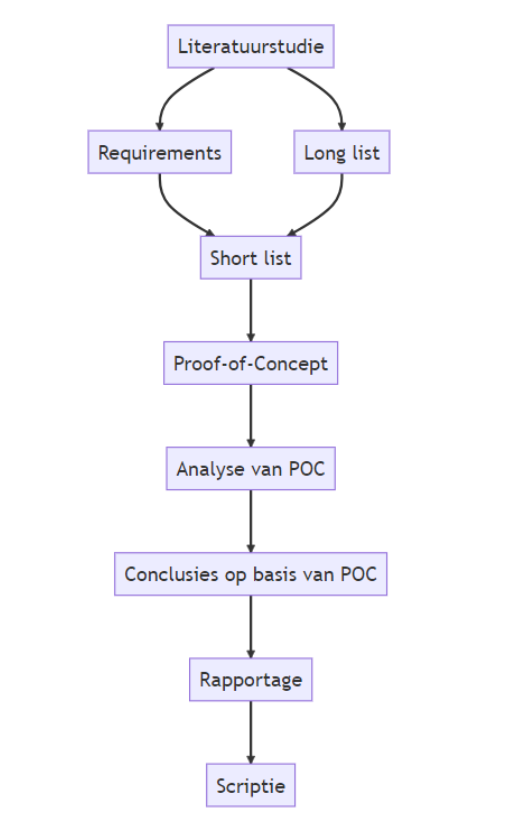
\includegraphics[width=0.7\linewidth]{img/flowchart}
  \caption{Flowchart}
  \label{fig:flowchart}
\end{figure}

Hieropvolgend wordt er een Proof-of-Concept (PoC) ontwikkeld en geïmplementeerd. Er zullen twee applicaties opgesteld worden, de een in React Native en de ander in Ionic. Voor Ionic zal er gekozen worden voor het framework React om een zo nauwkeurig mogelijk beeld te geven van de performantieverschillen tussen beide frameworks. Er zullen verschillende versies van de applicatie ontwikkeld worden met elk een andere focus. Zo kan er bijvoorbeeld gekeken worden naar de impact van de resolutie van videobeelden of hoe snel deze kunnen verwerkt worden binnen de framework. Voor het CPU-gebruik zullen profiler tools gebruikt worden om deze te meten. Dit kan aan de hand van React Devtools voor React Native en Chrome Devtools voor Ionic. Voor het geheugengebruik zal er verder gebruikt gemaakt worden van de Android Profiler in Android Studio. Tot slot zal er ook nog gekeken worden naar laadtijden van interessante invalshoeken uit de eerder opgestelde short list. Het is hierbij belangrijk dat er niet wordt gekeken naar hoe het apparaat omgaat met het afspelen van video's, maar wel hoe de frameworks omgaan met het ophalen en vervolgens verwerken van deze beelden tot deze begrijpbaar zijn voor de native video-compilers. Deze fase zal ongeveer 4-5 weken duren.

In de voorlaatste fase van de methodologie worden de resultaten van de PoC geanalyseerd en vergeleken. Hierbij wordt er gekeken naar de verschillen in performantie tussen beide frameworks. De nodige grafieken en tabellen zullen worden opgesteld om de resultaten te visualiseren. Deze fase zal ongeveer 1 week in beslag nemen.

Tot slot worden alle bevindingen gebundeld in een aaneensluitende scriptie. Deze zal een antwoord bieden op de centrale onderzoeksvraag. De uiteindelijke uiteenschrijving zal een drie- tot viertal weken in beslag nemen.

%---------- Verwachte resultaten ----------------------------------------------
\section{Verwacht resultaat, conclusie}%
\label{sec:verwachte_resultaten}

Het verwachte resultaat suggereert dat React Native vermoedelijk een kleine voorsprong zal hebben op Ionic voor de implementatie. Deze aanname heeft vooral te maken met de manier waarop React Native is opgebouwd. Zo maakt het gebruik van Native UI-elementen die rechtstreeks een positief effect zullen hebben op de compilatie en bijgevolg de performantie. 

